%----------------------------------------------------------------------------------------
%	CHAPTER 3
%----------------------------------------------------------------------------------------

\chapter{Opracowany algorytm}
\label{ch:opracowany-algorytm}
\chaptermark{Opracowany algorytm}
W przedstawionej pracy zrealizowano program rozpoznający tablice rejestracyjne na sekwencjach wideo pochodzących z kamery samochodowej.
Do detekcji użyto skanowania obrazu oknem przesuwnym i klasyfikowanie na podstawie cech Haara za pomocą algorytmu RealBoost.
Jako słaby klasyfikator wykorzystano algorytm koszykowania wartości funkcją logit.
Rozpoznane fragmenty obrazu zawierające tablice poddano operacjom morfologicznym.
Z przetworzonych obrazów segmentowano znaki tablicy rejestracyjnej.
Do rozpoznania znaków użyto biblioteki Tesseract opartej o rekurencyjne sieci neuronowe LSTM\@.


\section{Proces uczenia klasyfikatora}
\label{sec:proces-uczenia-klasyfikatora}
Proces uczenia klasyfikatora jest kluczowym etapem budowy modelu uczenia maszynowego.
Jeżeli na tym etapie dojdzie do błędu, będzie to rzutować na działanie całej aplikacji.
Częstym zjawiskiem w uczeniu maszynowym jest przeuczenie (ang. \textit{overfitting}).
Polega ono na wykrywaniu pozornych prawidłowości w dużej ilości danych, gdzie prawdziwe prawidłowości są prostsze lub słabsze, lub są maskowane przez błędy, lub są całkowicie nieistniejące~\cite{overfitting}.
Innym niepożądanym przypadkiem błędnego wyuczenia jest niedouczenie (ang. \textit{underfitting}).
Wynika ono najczęściej z zastosowania zbyt uproszczonego modelu lub niewystarczającej liczby próbek uczących~\cite{overfitting}.
Mając powyższe na uwadze, należy przyłożyć staranną uwagę do przygotowania odpowiedniego zbioru uczącego.
Nieprawidłowości na tym etapie będą bardzo trudno do wyeliminowania w późniejszych częściach systemu.

\subsection{Przygotowanie danych uczących}
\label{subsec:przygotowanie-danych-uczacych}
W rozdziale~\ref{ch:preparing_data_set} przedstawiono opracowany zbiór zdjęć z kamery samochodowej zawierający poruszające się pojazdy wraz z ich tablicami rejestracyjnymi.
Klasyfikatory działają jednak w inny sposób niż ludzki mózg i wymagają innych wartości, na których będą mogły podejmować decyzje.
W niniejszej pracy zdecydowano się wykorzystać cechy Haara jako cechy reprezentujące poszukiwane obiekty.
W celu wyuczenia klasyfikatora, należało opracowany wcześniej zbiór przetworzyć, aby każda negatywna i pozytywna próbka miała swoją reprezentację liczbową.
Na Rysunku~\ref{fig:haar_feats_dataset_prepare} przedstawiono schemat blokowy procesu przygotowania danych uczących dla klasyfikatora.
\begin{figure}[!ht]
    \centering
    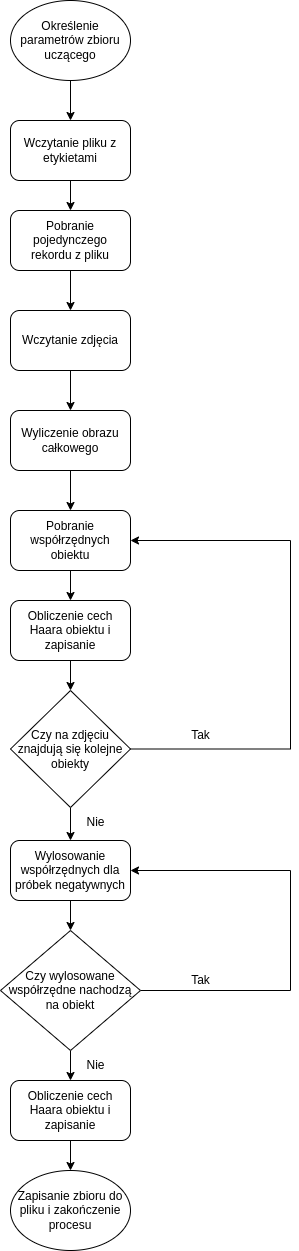
\includegraphics[scale=0.4]{Pictures/prepare_haar_dataset}
    \caption{Schemat blokowy przygotowania danych uczących dla klasyfikatora (źródło: opracowanie własne).}
    \label{fig:haar_feats_dataset_prepare}
\end{figure}
\FloatBarrier
Pierwszą czynnością jest określenie parametrów zbioru uczącego.
Przed rozpoczęciem uczenia należy określić ile cech ma być liczonych z jednej próbki.
Każdy szablon może być odpowiednią ilość razy skalowany wzdłuż każdego z kierunków.
Parametr ten oznacza się literą $s$.
Parametr $p$ oznacza rozmiary regularnej siatki ($(2p-1)\times (2p-1)$) punktów zaczepienia cech~\cite{szybka_detekcja_klesk}.
Na podstawie powyższych parametrów określa się liczbę cech niezbędnych do wyliczenia w trakcie przetwarzania jednego okna wg wzoru~\eqref{eq:features_count}
\begin{equation}
    \label{eq:features_count}
    n(s,p)=6s^2(2p-1)^2.
\end{equation}
Przykładowo, dla $s=3$ i $p=4$ liczba niezbędnych do wyliczenia cech jest równa 2205.
Dla $s=p=5$ liczba ta rośnie do 10125.
Im większa jest liczba cech tym dokładność detekcji powinna rosnąć.
Jednak wraz ze wzrostem liczby cech, rośnie również czas wykonania skryptu ze względu na większą liczbę niezbędnych do wykonania obliczeń.
Innym wejściowym parametrem jest ustalenie stosunku próbek pozytywnych do próbek negatywnych.

Po ustaleniu wejściowych parametrów, wczytywany jest plik tekstowy ze współrzędnymi tablic dla konkretnych plików.
Dla każdego rekordu w zbiorze, wczytywane jest odpowiednie zdjęcie.
Następnie algorytm iteruje po wszystkich pozytywnych próbkach znajdujących się w rozpatrywanym pliku.
Dla każdej próbki wyliczane są cechy Haara za pomocą wygenerowanych wcześniej szablonów.

W opisywanym programie użyto 5 szablonów cech Haara.
Szablony są skalowane odpowiednim skokiem zależnym od $s$.
Poniżej zamieszczono kod procedury generującej współrzędne szablonu dla każdej cechy~\ref{lst:haar_cords}.
\begin{lstlisting}[language=Python, caption=Procedura generujące szablony cech Haara dla konkretnych wpsółrzędnych., label={lst:haar_cords}]
def haar_coords(s, p, indexes):
    coords = []
    f_jump = (FEATURE_MAX - FEATURE_MIN) / (s - 1)
    for t, s_j, s_k, p_j, p_k in indexes:
        f_h = FEATURE_MIN + s_j * f_jump
        f_w = FEATURE_MIN + s_k * f_jump
        p_jump_h = (1.0 - f_h) / (2 * p - 2)
        p_jump_w = (1.0 - f_w) / (2 * p - 2)
        pos_j = 0.5 + p_j * p_jump_h - 0.5 * f_h
        pos_k = 0.5 + p_k * p_jump_w - 0.5 * f_w
        single_coords = [np.array([pos_j, pos_k, f_h, f_w])]  # whole rectangle for single feature
        for white in HAAR_TEMPLATES[t]:
            white_coords = np.array([pos_j, pos_k, 0.0, 0.0]) + white * np.array([f_h, f_w, f_h, f_w])
            single_coords.append(white_coords)
        coords.append(np.array(single_coords))
    return np.array(coords, dtype=object)
\end{lstlisting}
Na Rysunku~\ref{fig:haar_feats_examples} pokazano przykładowe szablony podczas procesu uczenia.
\begin{figure}[!ht]
    \centering
    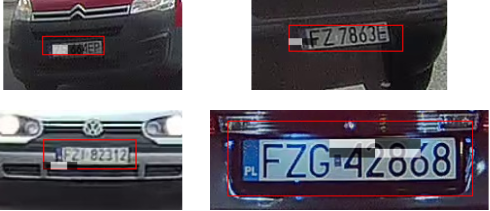
\includegraphics[scale=0.6]{Pictures/haar_tepmplates}
    \caption{Ekstrakcja cech za pomocą obrazów całkowych (źródło: opracowanie własne).}
    \label{fig:haar_feats_examples}
\end{figure}
\FloatBarrier

Po przeprocesowaniu wszystkich pozytywnych próbek, algorytm generuje negatywy.
Negatywne próbki są generowane losowo.
Losowana jest szerokość okna jako wartość w przedziale od 1 do 10 procent szerokości całego obrazu.
Wysokość okna jest zależna od szerokości.
Przyjęto, że wysokość okna powinna być równa $\dfrac{1}{3}, \dfrac{1}{4}$ lub $\dfrac{1}{5}$ szerokości.
Następnie dane są zapisywane do pliku.
W ten sposób przygotowane dane w następnym etapie posłużą do wyuczenia klasyfikatora.

\subsection{Uczenie klasyfikatora}
W niniejszej pracy zaimplementowano i wykorzystano algorytm wzmacniający RealBoost oparty o koszykowanie wartości funkcji logit.
Zasadę działania algorytmu RealBoost opisano szerzej w rozdziale~\ref{subsec:klasyfikatory}.
Na wejściu metody uczącej, funkcja przyjmuje cechy uczące oraz ich etykiety.
Dla każdej cechy obliczane są wartości maksymalne i minimalne.
Ustalane są one poprzez posortowanie wartości konkretnej cechy ze wszystkich próbek ze zbioru uczącego.
Algorytm dodaje odpowiedni margines, aby odrzucić skrajne wyniki.
Współczynnik ten ustalono na poziomie $0.05$.
Oznacza to, że dla zbioru o wielkości 100 próbek, odrzucone zostanie 5 pierwszych i 5 ostatnich wartości cech do wyznaczenia wartości brzegowych.
Następnie przypisywane są indeksy koszyków do poszczególnych cech.
Kolejnym krokiem jest przygotowanie indeksów, które przechowują informację o tym czy cecha dla konkretnego koszyka powiązana jest z próbką pozytywną czy negatywną.
Po przygotowaniu powyższych danych, algorytm przechodzi do wybrania najważniejszych cech z punktu widzenia klasyfikatora.
Obliczane jest to poprzez iterację po wszystkich cechach i określeniu cechy dla każdego klasyfikatora o najmniejszym błędzie.
Wyznaczane jest to za pomocą funkcji logit, która jest wyznaczana dla każdego z koszyków z osobna.
Na koniec dochodzi do reważenia wag.
Czynność jest powtarza dla każdego słabego klasyfikatora.
Algorytm~\ref{lst:fit_realboostbins} ukazuje fragment metody uczącej odpowiedzialny za wyliczenie odpowiedzi dla każdego ze słabych klasyfikatorów i wyznaczenie indeksów najlepszych cech.\\\\\\\\\\
\begin{lstlisting}[language=Python, caption=Procedura ucząca klasyfikator RealBoostBins., label={lst:fit_realboostbins}]
w = np.ones(m) / m
for t in range(self.T_):
    j_best = None
    logits_best = None
    err_exp_best = np.inf
    for j in range(n):
        logits = np.zeros(self.B_)
        for b in range(self.B_):
            W_positive = w[indexer_positive[j, b]].sum()
            W_negative = w[indexer_negative[j, b]].sum()
            logits[b] = self.logit(W_positive, W_negative)
        err_exp = np.sum(w * np.exp(-yy * logits[X_binned[:, j]]))
        if err_exp < err_exp_best:
            err_exp_best = err_exp
            logits_best = logits
            j_best = j
    self.feature_indexes_[t] = j_best
    self.logits_[t] = logits_best
    w = w * np.exp(-yy * logits_best[X_binned[:, j_best]])
    w /= err_exp_best

\end{lstlisting}
Na Rysunku~\ref{fig:fit_realboostbins} przedstawiono schemat blokowy uczenia klasyfikatora.
\begin{figure}[!ht]
    \centering
    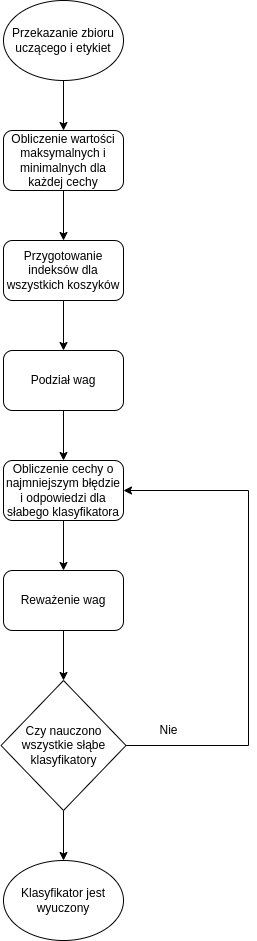
\includegraphics[scale=0.4]{Pictures/fit_realboostbins}
    \caption{Schemat blokowy funkcji uczącej klasyfikatora RealBoostBins (źródło: opracowanie własne).}
    \label{fig:fit_realboostbins}
\end{figure}
\FloatBarrier


\section{Schemat algorytmu}

Główną część programu można podzielić na dwa osobne moduły.
Pierwszy z nich odpowiedzialny jest za detekcję tablic na obrazie wejściowym.
Drugi moduł odpowiada za segmentację i rozpoznawanie znaków.
Przed rozpoczęciem detekcji, obraz jest skalowany.
W opracowanym algorytmie, ustalono wysokość na poziomie 480px.
Szerokość obrazu była proporcjonalnie skalowana.
Następnie obraz konwertowano do skali szarości.
Przed rozpoczęciem detekcji oknem przesuwnym, obliczano obraz całkowy.
Szablony cech Haara ograniczono tylko do tych odpowiadających cechom wybranym przez słabe klasyfikatory na etapie uczenia klasyfikatora.
Na Rysunku~\ref{fig:main_alg} przedstawiono schemat blokowy algorytmu rozpoznawania tablic rejestracyjnych.
\begin{figure}[!ht]
    \centering
    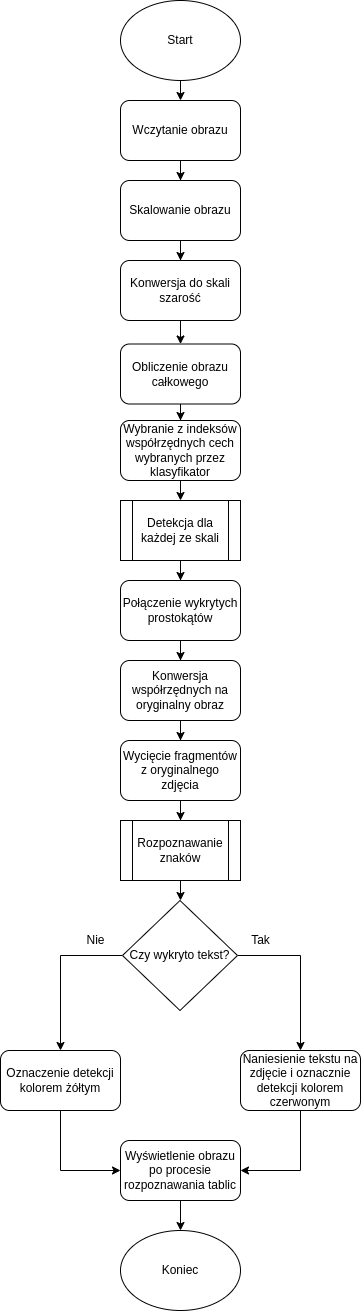
\includegraphics[scale=0.4]{Pictures/main_alg}
    \caption{Schemat blokowy algorytmu rozpoznawania tablic rejestracyjnych (źródło: opracowanie własne).}
    \label{fig:main_alg}
\end{figure}
\FloatBarrier

\subsection{Algorytm detekcji}
Algorytm detekcji odpowiada za zlokalizowanie obszarów potencjalnie zawierających tablice rejestracyjne.
Mając na uwadze fakt, że tablice mogą mieć różne rozmiary na zdjęciu, dla procedury skanującej oknem przesuwnym należało zastosować kilka skal okna.
Okno przesuwano w obrazie odpowiednim skokiem w poziomie oraz w pionie.
Poziomy skok $d_w$ obliczano na podstawie wzoru~\eqref{eq:jump_detect_window}
\begin{equation}
    \label{eq:jump_detect_window}
    d_w = \round(w * \lambda),
\end{equation}
gdzie $w$ jest szerokością okna, a $\lambda$ oznacza współczynnik przemieszczania okna.
Skok pionowy wyznaczano w analogiczny sposób.
Dla każdego okna obliczano cechy Haara dla indeksów wyznaczonych podczas procesu uczenia klasyfikatora.
Następnie obliczano odpowiedź klasyfikatora.
Jeśli była ona większa od podanego progu, okno oznaczano jako pozytywne.
Na Rysunku~\ref{fig:detection_alg} przedstawiono schemat blokowy algorytmu detekcji tablic rejestracyjnych.
\begin{figure}[!ht]
    \centering
    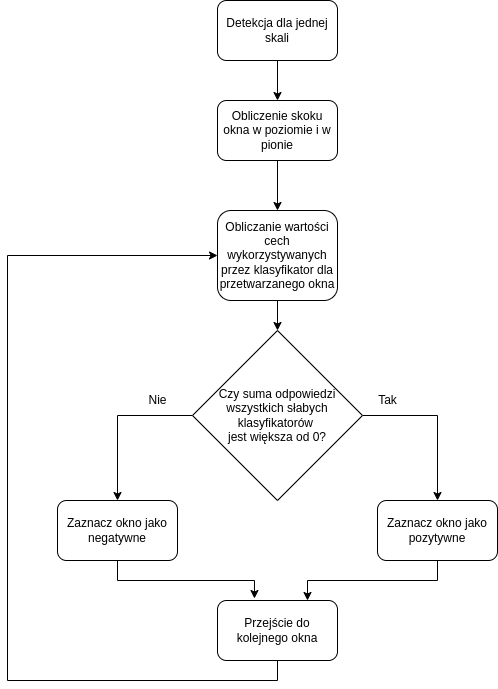
\includegraphics[scale=0.4]{Pictures/detection_alg}
    \caption{Schemat blokowy algorytmu detekcji tablic rejestracyjnych (źródło: opracowanie własne).}
    \label{fig:detection_alg}
\end{figure}
\FloatBarrier
Po wykonaniu procedury skanowania oknem przesuwnym, rozpoczęto przetwarzanie okien oznaczonych jako pozytywne.
Z uwagi na fakt, że w otoczeniu tablicy rejestracyjnej wiele okien mogło zostać oznaczonych jako pozytywne, należało te okna połączyć.
Dzięki temu moduł rozpoznawania znaków otrzyma znacznie mniejszą ilość okien.
W kolejnym kroku współrzędne połączonych okien konwertowano do współrzędnych w oryginalnym obrazie.
Taka operacja ma na celu przekazanie do modułu OCR fragmentu obrazu w jakości równej obrazowi sprzed procedury skalowania.
Rysunek~\ref{fig:non_max_supression} przedstawia porównanie procedury detekcji bez oraz z zastosowaniem techniką łączenia okien.
Do połączenia okien zastosowano algorytm usuwania niemaksymalnych pikseli (ang. \textit{non-maximum suppression}).
\begin{figure}[!ht]
    \centering
    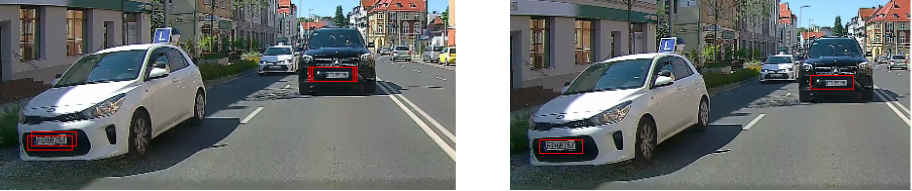
\includegraphics[scale=0.4]{Pictures/non_max_supression}
    \caption{Porównanie detekcji tablicy rejestracyjnej bez i z zastosowaniem algorytmu łączenia okien (źródło: opracowanie własne).}
    \label{fig:non_max_supression}
\end{figure}
\FloatBarrier

\subsection{Algorytm segmentacji i rozpoznawania znaków}
Moduł odpowiedzialny za rozpoznawanie znaków otrzymuje na wejściu wycięty fragment obrazu w oryginalnej jakości.
Następnie przed rozpoczęciem segmentacji znaków, obraz jest skalowany do wysokości 300px.
W kolejnym kroku, obraz jest konwertowany do modelu barw w skali szarości.
W celu segmentacji znaków, zaproponowano podejście łączące dwie techniki.
Zdecydowano się na takie rozwiązanie, ponieważ zauważono, że wzajemnie się one uzupełniają i ich połączenie daje lepsze wyniki.
Pierwsza z technik polegała na binaryzacji obrazu z wykorzystaniem metody Otsu.
Na tak przygotowanym obrazie wykryto kontury korzystając z metody z biblioteki OpenCV \textit{findContours}.
Druga technika wykorzystywała maskę binarną w przestrzeni barw HSV\@.
Następnie przetworzony obraz poddawano operacjom morfologicznym.
Wynikowy obraz przekazano do metody wykrywającej kontury.

Metoda \textit{findContours} przyjmuje parametr $mode$, który odpowiada za sposób selekcji konturów.
Procedura może zwracać np.\ tylko kontury zewnętrzne lub wewnętrzne lub zwracać strukturę hierarchiczną~\cite{open_cv_contours_mode}.
W opisywanym rozwiązaniu wybrano opcje \textit{RETR\_TREE}, która pobiera wszystkie kontury i rekonstruuje pełną hierarchię zagnieżdżonych konturów.
W \textit{findContours} możliwa jest również do wybrania metoda aproksymacji konturów.
Dla wartości \textit{CHAIN\_APPROX\_NONE} zbierane są wszystkie wartości konturów.
Dla wartości \textit{CHAIN\_APPROX\_SIMPLE} algorytm kompresuje poziomie, pionowe oraz diagonalne segmenty i pozostawia tylko punkty końcowe.
Zdecydowano się na drugą metodę aproksymacji.

Dla obu podejść zbiory wykrytych konturów połączono w całość.
Wykryte kontury należało przefiltrować, w celu wybrania tylko tych odpowiadającym znakom na tablicy rejestracyjnej.
Opracowano procedurą z następującymi krokami:
\begin{enumerate}
    \item pobranie prostokąta otaczającego dany kontur,
    \item odrzucenie konturu, jeśli wysokość prostokąta jest większa od wysokości obrazu pomniejszonej o stałą wartość
    \item obliczenie powierzchni prostokąta,
    \item odrzucenie konturu, jeśli powierzchnia jest mniejsza od stałej wartości,
    \item odrzucenie konturu, jeśli stosunek boków prostokąta jest spoza przyjętego zakresu.
\end{enumerate}
Na podstawie powyższej procedury odrzucono część wykrytych wcześniej konturów.
Korzystając z założenia, że wszystkie znaki na tablicy rejestracyjnej są takiej samej wysokości, odrzucono z powstałego zbioru kontury, których wysokość najbardziej odbiegała od średniej wysokości całego zbioru.
Ostateczny zbiór konturów posłużył do wycięcia znaków ze zbinaryzowanego obrazu.
W ten sposób przeprowadzono segmentację znaków.
Nowy obraz, z oddzielonymi znakami od tła, przekazano do biblioteki Tesseract.
Skorzystano z metody \textit{image\_to\_string}, która zwraca tekst na podstawie obrazu wejściowego.
Na Rysunku~\ref{fig:characters_alg} przedstawiono schemat blokowy algorytmu rozpoznawania znaków.
\begin{figure}[!ht]
    \centering
    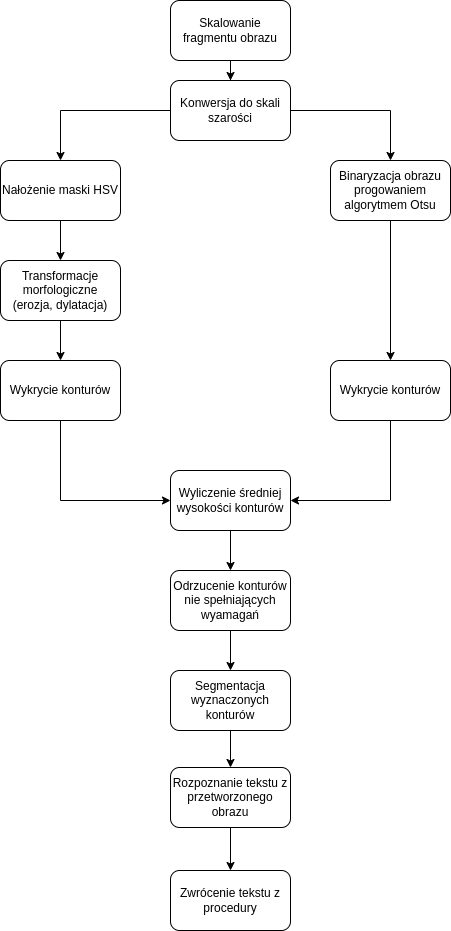
\includegraphics[scale=0.4]{Pictures/characters_alg}
    \caption{Schemat blokowy algorytmu rozpoznawania tablic (źródło: opracowanie własne).}
    \label{fig:characters_alg}
\end{figure}
\FloatBarrier
Na Rysunku~\ref{fig:segmentation} przedstawiono przykładowy proces segmentacji znaków.
Pierwszy obraz jest obrazem wejściowym, który trafił do algorytmu z detektora tablic rejestracyjnych.
Ostatni obraz jest wynikiem segmentacji.
Obraz środkowy jest obrazem wejściowym, na który nałożono wykryte pozycje znaków (kolor niebieski).
Kolorem różowym oznaczono kontury, które zostały wykryte, ale zostały odrzucone z powodu braku spełnienia kryteriów geometrycznych.
Założono, że kontur musi być prostokątem o dłuższych bokach zorientowanych w pionie.
Kolorem żółtym oznaczono kontury, które zostały odrzucone, z powodu ich zbyt dużego odchylenia od średniej wysokości konturów.
\begin{figure}[!ht]
    \centering
    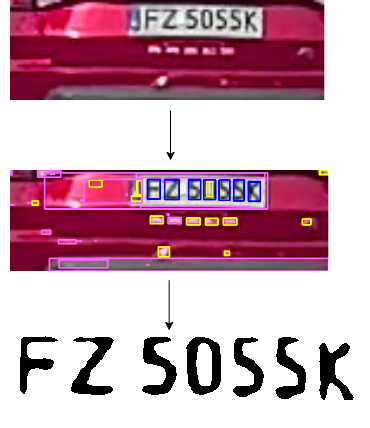
\includegraphics[scale=0.4]{Pictures/segmentation}
    \caption{Proces segmentacji znaków (źródło: opracowanie własne).}
    \label{fig:segmentation}
\end{figure}
\FloatBarrier


\section{Biblioteki użyte w programie}
Środowisko Python jest niezwykle popularne m.in. ze względu na mnogość dostępnych gotowych bilbiotek.
Jednym z celów pracy było zaimplementowanie algorytmu uczącego i klasyfikującego.
Cel ten udało się zrealizować, natomiast nie byłoby to możliwe bez użycia gotowych rozwiązań do elementarnych operacji t.j. listowanie plików w katalogach, odczyt i zapis zdjęć, pobieranie pojedynczych klatek z filmu wideo czy operacje na tablicach.
Poniżej wymieniono i opisano najważniejsze oraz najczęściej używane biblioteki w opisywanej pracy.

\subsection{OpenCV}
OpenCV jest biblioteką o otwartym źródle (ang. \textit{open source}) \cite{open_cv,open_cv_docs} .
Do jej głównych zastosowań należą przetwarzanie obrazów oraz uczenie maszynowe.
W przedstawionym programie wykorzystano najnowszą dostępną wersję na moment pisania pracy $4.6.0$.
Została zaprojektowana, aby zapewnić ustandaryzowaną infrastrukturę dla aplikacji widzenia komputerowego.
Oprogramowanie dystrybuowane jest na licencji BSD.
Pierwsza wersja została opracowana w roku 1999.
Oryginalnie powstała w języku C++, natomiast istnieją biblioteki pozwalające używać jej w innych językach programowania.
Bibliotekę można podzielić na kilka głównych modułów:
\begin{itemize}
    \item przetwarzanie obrazów - moduł zawiera zestaw metod do przeprowadzania takich operacji jak filtrowanie, przekształcenia geometryczne, zmiana przestrzeni kolorów, histogramy,
    \item przetwarzanie wideo - zestaw metod, które pozwalają na m. in. usuwanie tła, śledzenie obiektów, wykrywanie ruchu,
    \item operacje wejścia/wyjścia na wideo - wyciąganie poszczególnych klatek z wideo, kodowanie, zapis i odczyt wideo,
    \item HighGUI - moduł służący do wizualizacji wyników, wyświetlania okien, zaznaczania ROI (ang. \textit{Region of interest}).
\end{itemize}

Poniżej wymieniono użyte w stworzonym programie funkcje wraz z krótkim opisem ich zastosowania:
\begin{itemize}
    \item \textit{videoCapture} - przechwytywanie obrazów z pliku wideo,
    \item \textit{cvtColor} - zmiana przestrzeni barw w obrazie,
    \item \textit{imread} - wczytanie obrazu z pliku,
    \item \textit{imshow} - wyświetlenie obrazu,
    \item \textit{imwrite} - zapis obrazu do pliku,
    \item \textit{rectangle} - rysowanie prostokąta na obrazie,
    \item \textit{putText} - umiejscowienie tekstu na obrazie,
    \item \textit{addWeighted} - połączenie dwóch obrazów poprzez nałożenie ich na siebie,
    \item \textit{thresholding} - binaryzacja obrazu,
    \item \textit{GaussianBlur} - wygładzanie obrazu za pomocą funkcji Gaussa,
    \item \textit{Canny} - wykrywanie krawędzi za pomocą algorytmu Johna F. Canny'ego \cite{4767851},
    \item \textit{findContours} - wykrywanie konturów obiektów (punktów o tym samym kolorze lub intensywności łączących się w krzywe),
    \item \textit{resize} - zmiana wielkości obrazu,
    \item \textit{imdecode} - odczytywanie zdjęcia z bufora.
\end{itemize}

\subsection{Tesseract OCR}
Biblioteka Tesseract jest pakietem składającym się z programu lini poleceń \textit{tesseract} oraz silnika OCR \textit{libtesseract}~\cite{tesseract}.
Tesseract powstał między rokiem 1985, a 1994 na potrzeby firmy Hewlett-Packard.
W roku 2005 firma upubliczniła bibliotekę jako rozwiązanie \textit{open-source}.
Od początku 2006 do listopada 2018 za rozwój Tesseract odpowiedzialna była firma Google.
Obecnie głównym programistą projektu jest Ray Smith.
Silnik programu oparty jest o język programowania C++.
W celu wykorzystania jej w opisywanym programie, użyto nakładki \textit{pytesseract}~\cite{pytesseract}.
Autorzy deklarują, że najnowsza wersja 5, wydana w listopadzie 2021, wspiera ponad 100 języków.
Biblioteka wykorzystuje rekurencyjne sieci neuronowe LSTM (ang. \textit{Long Short-Temp Memory})~\cite{lstm}.

\subsection{Numpy}
TODO

\subsection{Pickle}
TODO

\subsection{Numba}
Biblioteka od przyspieszania kodu (jit)